\section{Conventional \ac{1D} datasets}
\label{sec:evaluation}

As discussed in \cref{subsec:phase-variance}, one of the disadvantages of
\ac{SVD}-based methods like the \ac{MPM} is their propensity to generate
parameter estimates featuring oscillators with spurious phase behaviour. Such
behaviour is most prevalent in \acp{FID} featuring signals with very similar
frequencies, and low \ac{SNR}. To assess the ability of the inclusion of the
\ac{NLP} routine to produce improved parameter estimates\footnote{
    ``Improved'' in this context means ``in better agreement with the
    underlying phenomenon leading to the dataset''. A given set of parameters
    may fit the data well in a \ac{RSS} sense, but this doesn't necessarily
    imply the it confers meaning on the sample of interest on a per-signal
    level.
}, comparisons are now made between results generated with the \ac{MPM} in
isolation, and with the inclusion of phase variance-regularised \ac{NLP}. For
the experimental datasets considered, the data was pre-processed using
\textsc{Bruker}'s \textsc{TopSpin} software, using the series of commands
\texttt{ft; pk; abs}, which perform \ac{FT}, automatic phase correction, and
baseline correction, respectively. The data was then converted back to the
time-domain using \ac{IFT}.

\subsection{``Twenty signals''}
\begin{sidewaysfigure}
    \centering
    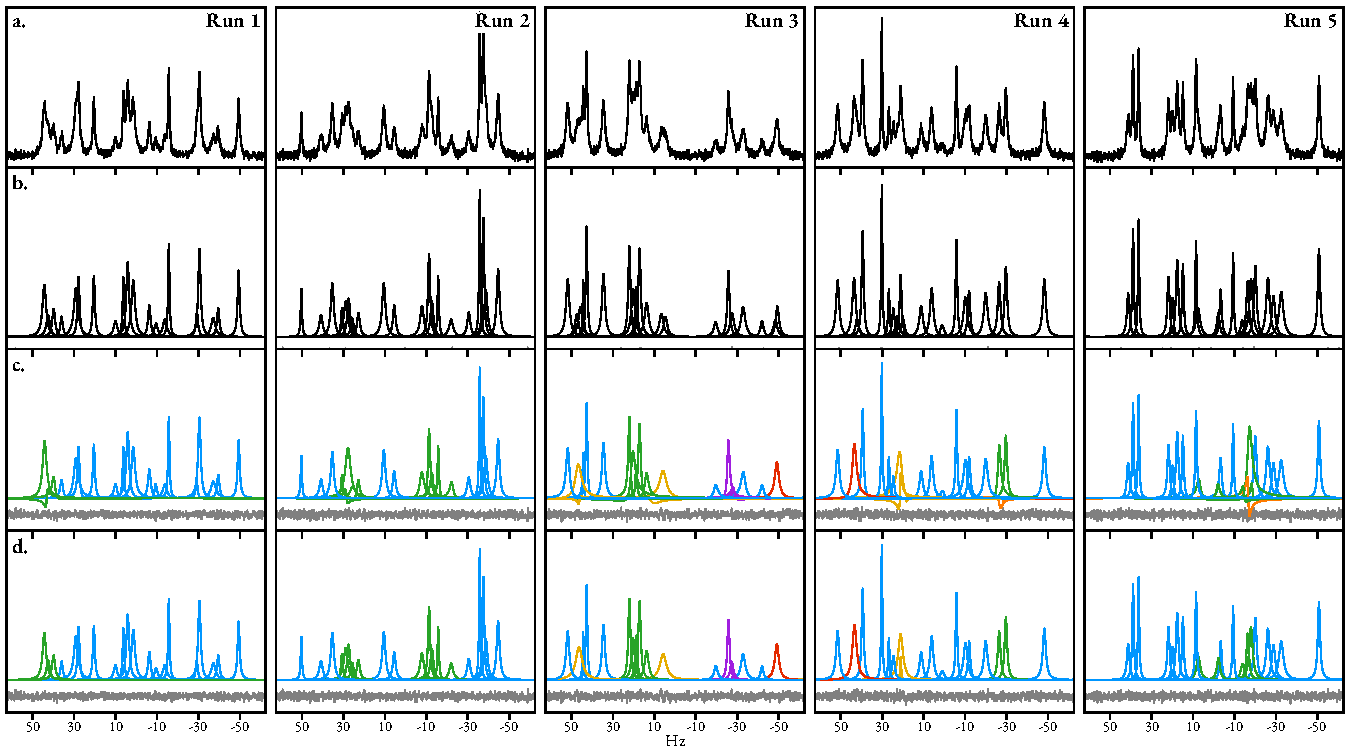
\includegraphics{mpm_vs_nlp/mpm_vs_nlp.pdf}
    \caption[
        The result of estimating a series of 5 simulated signals comprising 20
        oscillators, using solely the \acs{MPM} and also with phase
        variance-regularised \acs{NLP} afterwards.
    ]{
        The result of estimating a series of 5 simulated signals comprising 20
        oscillators (see the main text for details on how the datasets were constructed).
        \textbf{a.} Spectra of the datasets generated.
        \textbf{b.} Spectral lines corresponding to the true set of oscillators
        used to generate each dataset.
        \textbf{c.} Plots of peaks for each oscillator generated using
        the \acs{MPM}.
        \textbf{d.} An equivalent plot for the result after applying \acs{NLP},
        with the \acs{MPM} result being the initial guess.
        Also included in \textbf{c.} and \textbf{d.} is the residual between the
        data and the sum of the oscillator peaks (grey line).
        The colouring of oscillator lines in \textbf{c.} and \textbf{d.} is
        described in the main text.
    }
    \label{fig:mpm_vs_nlp}
\end{sidewaysfigure}
A series of five simulated \acp{FID} were constructed using
\cref{eq:hypercomplex-fid} with $D=1$. For each \ac{FID}, a model order
of $M=20$ was used, the number of points sampled was $N = 1024$, the sweep
width was $\fsw=\qty{125}{\hertz}$, and the transmitter offset was $\foff
= \qty{0}{\hertz}$.  Each oscillator was assigned a phase of \ang{0}, while the
amplitudes, frequencies and damping factors were drawn at random from the
following distributions:
$a_m \sim \mathcal{U}(1, 5)$, $f_m \sim \mathcal{U}(\qty{-55}{\hertz},
\qty{55}{\hertz})$, $\eta_m \sim \mathcal{U}(\qty{2}{\per\second},
\qty{8}{\per\second})\ \forall m \in \lbrace 1, \cdots, 20\rbrace$. An extra
constraint was applied to the frequencies,
such that no two oscillators were permitted to have frequencies that differed
by less than $\nicefrac{4 \fswone}{\None} \approx \qty{0.49}{\hertz}$. Each
noiseless \ac{FID} $\bx$ was then corrupted with \ac{AWGN}, with a target
\ac{SNR} of \qty{25}{\deci\bel}, with the noise variance for each signal
determined using the equation
\begin{equation}
    \sigma^2 = \frac{1}{20^{2.5} N}
        \sum_{n=0}^{N-1} \lvert x_n \rvert^2.
\end{equation}
The spectra of the simulated \acp{FID} are presented in panel a of
\cref{fig:mpm_vs_nlp}, with the true set of oscillator peaks which contribute
to the spectrum in panel b. With the criteria used, it can be seen that such
datasets feature signals which often suffer from severe overlap, with the high
noise variance compounding the opportunity to clearly identify all contributing
signals.

For each \ac{FID}, the \ac{MPM} was performed, assuming that the model order is
30, constituting a considerable over-fit. The \ac{MDL} tended to produce
considerable under-estimates of $M$ when applied to these \acp{FID}, so the
hard-coded value was used instead. When an excessive model order is provided to
the \ac{MPM}, it is typical that oscillators corresponding to the noise
subspace of the data matrix $\Hy$ are characterised by small amplitudes and/or
very small damping factors. For this reason, prior to subjecting the \ac{MPM}
result to \ac{NLP}, oscillators which satisfied either $a_m < 0.1$ or  $\eta_m
< \qty{0.7}{\per\second}$ were removed from the parameter set. The individual
oscillators which make up the \ac{MPM} result after purging spurious components
are displayed in panel c of \cref{fig:mpm_vs_nlp}, along with the residual
between the data and the summation of all the oscillator peaks.

The \ac{MPM} invariably generates a model with good agreement with the data as
a whole, as evidenced by the residual.
However, it can be seen that in several spectral regions across the datasets,
especially ones that are highly crowded, oscillators possess parameters which
deviate significantly from the true ones.
Most notably, individual oscillator phases regularly stray far from \ang{0},
and their associated amplitudes are often considerably different too.
In panel c of \cref{fig:mpm_vs_nlp}, the blue oscillators are those which
agree very closely with a particular ``true signal'' in the data.
Oscillators with other colours are not clearly mapped to a true signal,
with the different colourings described shortly.
The intention is for the \ac{NLP} routine to adjust the parameters describing
the non-blue oscillators in panel c such that they agree with true signals,
while having little to no effect on the blue oscillators. The results of
\ac{NLP} are provided in panel d.

In discussing the outcome of the routine, it will be useful to introduce the
concept of a \emph{frequency neighbourhood}, a loose term which describes a
small, continuous range of frequencies within the spectral window. As the
\ac{NLP} routine involves taking small steps
through parameter space in an attempt to converge, it is unlikely that an
oscillator which starts off with a frequency far away from a particular
frequency neighbourhood will eventually enter it. As such, in order for the
\ac{NLP} routine to successfully estimate the region, sufficient oscillators
need to present within the neighbourhood in the first place. Cases where the
\ac{MPM} generated enough oscillators for a given frequency neighbourhood,
albeit with parameters which are noticeably off the true parameters are in
either green or yellow. Green oscillators are those which the \ac{NLP} routine
was able to adjust in order to achieve agreement with the true result. As such,
they indicate improvements to the estimation result as opposed to the \ac{MPM}
being used by itself. Conversely, yellow oscillators denote cases where, though
sufficient oscillators exist in the frequency neighbourhood in the initial
guess, the \ac{NLP} routine evolves such that at least one of the oscillators
is driven by the phase variance constraint to acquire a negative amplitude,
leading to it being purged from the parameter set. This typically occurs when an
oscillator has an initial phase which is considerably greater than
$\nicefrac{\pi}{2}$\,\unit{\radian}.
Yellow oscillators therefore indicate cases where the final result has
under-fit the dataset. There are a few instances, denoted by red oscillators,
where the \ac{MPM} assigned too few oscillators to a particular frequency
neighbourhood, and as such the \ac{NLP} would not have been able to yield any
improvement. This typically occurs with what can safely be described as
fiendishly difficult cases, where severe signal overlap and low \ac{SNR} make
it very difficult to associate certain spectral regions with more than one
signal by eye.
The final two oscillator groupings, denoted by purple and orange, denote cases
where the \ac{MPM} generated more oscillators than are present in a given
frequency neighbourhood (i.e. the data was over-fit in this region). Orange
oscillators we purged by the \ac{NLP} routine due to their acquiring negative
amplitudes. This enabled a parsimonious fit of the frequency neighbourhood by
the oscillators which remained. Finally, the purple oscillators denote the one
occasion (Run 3) where an over-fit occurred, and the model order was not
successfully reduced by the \ac{NLP} routine. One of the purple oscillators in
the \ac{MPM} appears to agree closely with a significant ``blip'' in the noise.
The over-fit has therefore occurred because this noise component was
incorporated into the final result; it was neither purged based on the
amplitude and damping factor criteria outlined above, nor by acquiring a
negative amplitude during \ac{NLP}.

\subsection{Andrographolide}
\begin{sidewaysfigure}
    \centering
    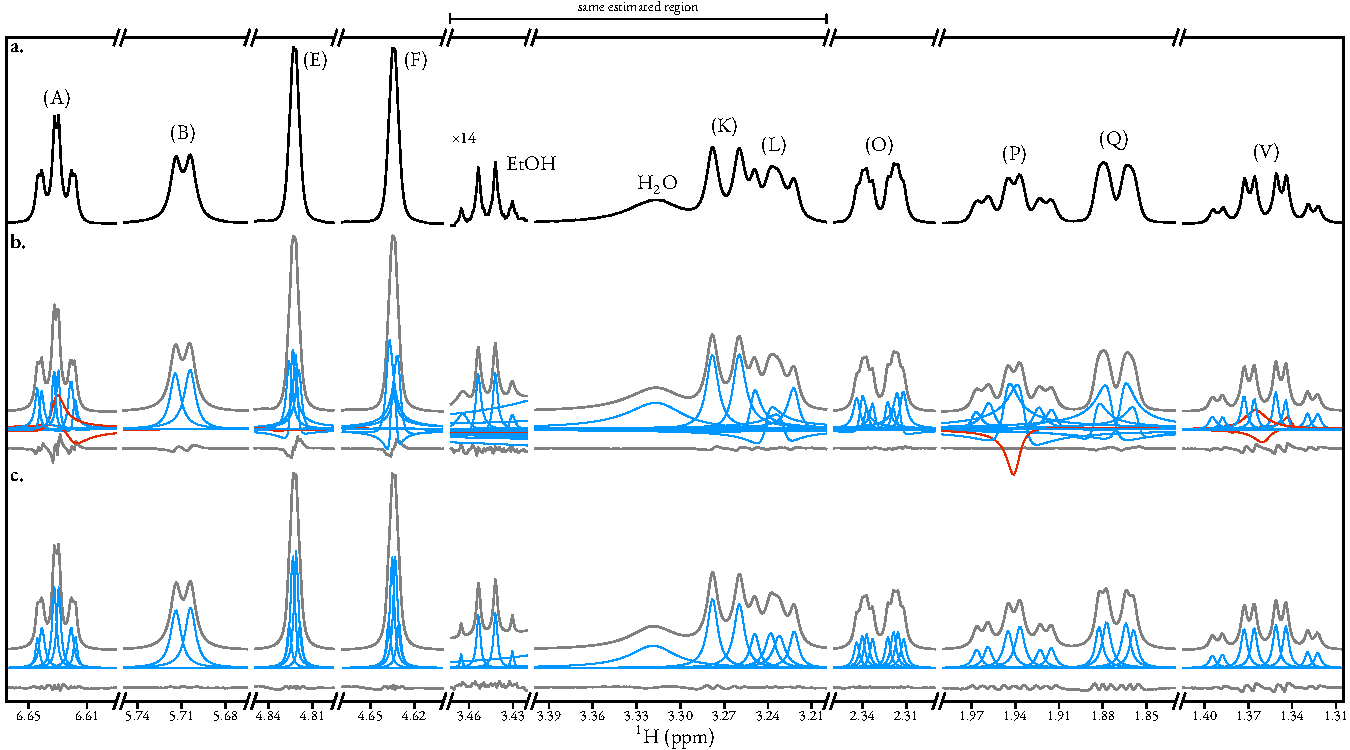
\includegraphics{andrographolide_onedim/andrographolide_onedim.pdf}
    \caption[
        Result of applying the estimation routine to selected regions of a
        pulse-acquire dataset of andrographolide.
    ]{
        Result of applying the estimation routine to selected regions of a
        pulse-acquire dataset of andrographolide in \acs{DMSOd6}.
        \textbf{a.} Spectral data corresponding to the regions considered.
        \textbf{b.} The result of applying the \acs{MPM} to the regions, with
        the model order predicted with the \acs{MDL}. Blue/red lines: peaks of
        individual oscillators, grey line above: the model (sum of all
        oscillators), grep line below: the residual between the data and the model.
        \textbf{c.} The result after convergence of the \acs{NLP} routine, again
        with the model above and residual below.
        Red peaks in panel b correspond to oscillators which acquire negative
        amplitudes during the \acs{NLP} routine, and are subsequently purged.
        Note that one of the reasons estimated has been split in two in the
        figure to save space, with one half, featuring a signal from ethanol,
        being magnified.
    }
    \label{fig:andro-onedim}
\end{sidewaysfigure}
\Cref{fig:andro-onedim} illustrates the outcome of applying the
estimation routine to selected regions of a \textsuperscript{1}H dataset of
andrographolide (\cref{fig:structures}.e) in \acs{DMSOd6}, acquired with
a \qty{600}{\mega\hertz} spectrometer.
The \ac{NLP} routine is effective at resolving the spurious phase-behaviour
often generated by the \ac{MPM} (cf. panels b and c).
It's ability to estimate parameters from resonances with high
dynamic range and high variation of damping factors is also evidenced by the
fact that it was able to assign an intense broad singlet, corresponding to
water which has entered the sample over time, alongside a nearby quartet
corresponding to the methylene of some residual ethanol in the sample.
For some of the sub-\acp{FID} considered, the \ac{MPM} also featured certain
oscillators\,---\,commonly with very high damping factor and/or phases far from
\ang{0}\,---\,which ended up being purged by the \ac{NLP} routine (see the red
peaks in panel b). As a result of purging these oscillators, and ensuring
consistent phases across oscillators, routine does well at generating parameter
estimates which describe the apparent multiplet structures associated with each
spin. \Cref{tab:andro-multiplets} provides an overview of the most significant
couplings associated with the spins giving rise to the multiplet structures
considered.
\begin{table}
\centering
\begin{tabular}{c c c}
\hline
Spin  & Coupling partners & Multiplet structure \\
\hline
\multicolumn{3}{c}{\textbf{Andrographolide}}\\
\hline
(A) & (D)\textsuperscript{long}, (M)\textsuperscript{vic}, (N)\textsuperscript{vic} & ddd (\emph{dt}) \\
(B) & (D)\textsuperscript{ex} & d \\
(E) & (F)\textsuperscript{vinyl}, \dots & d\dots \\
(F) & (E)\textsuperscript{vinyl}, \dots & d\dots \\
(K) & (J)\textsuperscript{gem}, (H)\textsuperscript{ex} & d \\
(L) & (C)\textsuperscript{ex}, (T)\textsuperscript{180}, (U)\textsuperscript{60} & dd \\
(O) & (P)\textsuperscript{gem}, (R)\textsuperscript{60}, (V)\textsuperscript{60} & ddd \\
(P) & (O)\textsuperscript{gem}, (R)\textsuperscript{60}, (V)\textsuperscript{180} & ddd (\emph{dt}) \\
(Q) & (M)\textsuperscript{vic}, (N)\textsuperscript{v}, \dots & dd\dots \\
(V) & (O)\textsuperscript{60}, (P)\textsuperscript{180}, (R)\textsuperscript{g}, (W)\textsuperscript{180} & dddd (\emph{dq}) \\
\hline
\multicolumn{3}{c}{\textbf{Cyclosporin A}}\\
\hline
(A) & diastereotopic pair on \textsuperscript{\textbeta}C & dd \\
(B) & ---''--- & dd \\
(C) & ---''--- \& amide proton & ddd (\emph{dt}) \\
(D) & proton on \textsuperscript{\textbeta}C \& amide proton & dd \\
(E) & methyl protons on \textsuperscript{\textbeta}C \& amide proton & dq \\
(F) & ---''--- & dq (\emph{quintet}) \\
\hline
\end{tabular}
\caption[
    Major coupling partners associated with spins in andrographolide and
    cyclosporin, considered in \cref{fig:andro-onedim,fig:cyclosporin}
    respectively, along with the multiplet structures that arise.
]{
    Major coupling partners associated with spins in andrographolide and
    cyclosporin, considered in \cref{fig:andro-onedim,fig:cyclosporin}
    respectively, along with the multiplet structures that arise.
    For andrographolide, coupling partners are labelled as follows:
    \textsuperscript{vinyl} geminal coupling between two vinylic protons,
    \textsuperscript{ex} geminal coupling between two protons, in which one
    is bonded to an oxygen, leading to exchange decoupling\cite[Section
    2.6.1.5]{Claridge2016},
    \textsuperscript{gem} geminal coupling,
    \textsuperscript{long} long-range coupling,
    \textsuperscript{vic} vicinal coupling,
    \textsuperscript{60} geminal coupling, with a fixed dihedral angle of \ang{60},
    \textsuperscript{180} geminal coupling, with a fixed dihedral angle of \ang{180}.
    All cyclosporin couplings of significance are geminal couplings.
    In cases where the observed multiplet structure is different to the true
    structure, the observed structure is is in brackets. Ellipses denote cases
    where more (long-range) coupling partners are likely, based on the
    estimation result generated, though these have not been explicitly determined.
}
\label{tab:andro-multiplets}
\end{table}

One of the most challenging aspects of estimating \ac{NMR} signals is
the fact that data frequently contains individual signals with incredibly
similar frequencies due to the effect of scalar couplings. Molecules
with fused ring systems such as andrographolide are prime examples of spin
systems which generate such datasets, as they tend to have very dense coupling
networks leading to complex multiplet structures. Also, fused systems often
exhibit appreciable long-range couplings (between spins separated by four or
more bonds) alongside more prevalent two-bond (geminal) and three-bond
(vicinal) couplings. Long range couplings can be particularly challenging to
resolve, as they are often of a comparable magnitude to the spectral resolution
($\nicefrac{\fsw}{N}$), so individual signals are barely perceptible.

Take the multiplet structure from spin (Q) as an example.
This has separate vicinal couplings to the
diastereotopic protons (M) and (N), which are likely the greatest magnitude couplings
associated with (Q). If these were the only couplings, a doublet of doublets
(dd) structure would be expected, which is what has been generated by
the estimation routine (see panel c in the region
\SIrange{1.85}{1.9}{\partspermillion}). However, a comparison of the data and
the model indicates that there is a clear discrepancy between the two,
evidenced by systematic ``wiggles'' in the residual. This feature hints at an
under-fit of the multiplet structure.
The \ac{MPM} generated oscillators with phases deviating far from \ang{0},
which enabled good agreement with the data in a residual sense, though of
course such a set of oscillators is unrealistic describing for a well-phased
\ac{FID}.
Long-range couplings with magnitudes that are large enough to influence the
appearance of (Q)'s multiplet structure are likely to be present, which leads
to a signal in which all contributing resonances are too poorly resolved to
realistically gleam any further meaningful information, at least at the field
strength used.

As a second illustration, the signal corresponding to spin (V) is also
under-fit, this time because the presence of a number of couplings of similar
magnitudes leads to resonances coalescing at roughly the same frequency; a
multiplet structure featuring 16 resonances forming in a ``dddd'' structure is
expected, however 3 of the couplings are of similar magnitudes, such that
individual resonances coalesce to form what is apparently a quartet of doublets (dq).
The estimation routine was able to resolve this dq structure,
however the large wiggles in the residual again imply that under-fitting has
occurred, and each oscillator is in fact being used to fit two or more
signals present in the \ac{FID}. Again, at the field strength used to
acquire the \ac{FID}, it is unlikely that an accurate resolution of all 16
oscillators by estimation is feasible.

At this point, rather the cause of large residual values being cause by
under-fitting, one may question whether the underlying model is actually suited
to describe the data.
There is for example precedent for fitting oscillators with non-exponential
decay profiles\,---\,profiles which lead to Voigt and Gaussian spectral
lineshapes are common\,---\,to improve the model fit\cite{Sima2007}.
However, for some multiplet structures in Figure \ref{fig:andro-onedim},
exceptionally good agreement between the model and data are made, using a
parsimonious set of parameters.
With three couplings of different magnitude, spin (O) exhibits a ``ddd''
multiplet structure in which all 8 signals are discernible. The \ac{NLP}
routine has performed effectively in taking the initial guess from the
\ac{MPM}\,---\,featuring the correct number of oscillators albeit with
spurious phases\,---\, and generating a well-phased set of oscillators defining
the ddd structure.

\note{Discussion of more challenging regions? Probably beyond the scope of the
routine without further user input/maybe just too difficult full stop?}

\subsection{Cyclosporin A}
\begin{figure}
    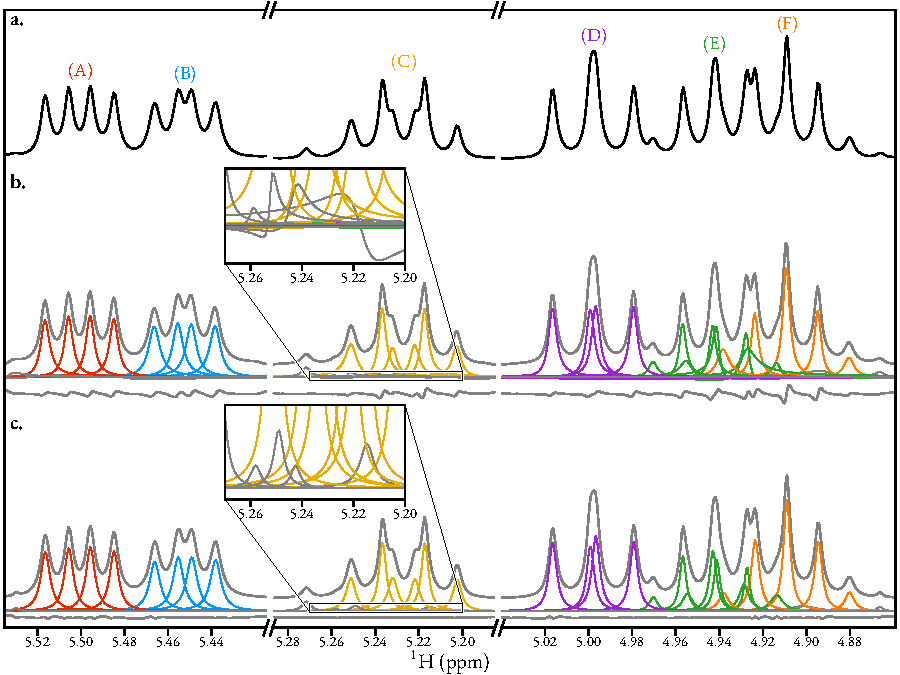
\includegraphics{cyclosporin/cyclosporin.pdf}
    \caption[
        Result of applying the estimation routine to selected regions of a
        pulse-acquire dataset of cyclosporin A.
    ]{
        Result of applying the estimation routine to selected regions of a
        pulse-acquire dataset of cyclosporin A in benzene-d\textsubscript{6}.
        The figure is of a similar layout to \cref{fig:andro-onedim}.
        Coloured peaks correspond to oscillators which have been assigned
        to multiplet structures of known spins. Grey oscillators correspond to
        those with an unknown association to a particular spin.
    }
    \label{fig:cyclosporin}
\end{figure}
The estimation routine was also applied to filtered sub-\acp{FID} from a
\proton\ pulse-acquire dataset of cyclosporin A \note{Structure in
appendix}\,---\, a cyclic peptide comprising 11 amino acids\,---\,in
benzene-d\textsubscript{6}. The regions considered all contain signals caused
by protons bound to C\textsuperscript{\textalpha} atoms in the peptide
backbone\cite{Verma2018}.
Particular challenges in estimating this dataset are (a) the presence of
heavily overlapping signals, most notably in the
\SIrange{5.02}{4.88}{\partspermillion} region, and (b) the presence of low
intensity ``nuisance'' signals, likely from impurities in the sample.

Nevertheless, the routine has performed effectively in generating a parameter
estimate which agrees with the multiplet structures present. For the most
downfield region considered, the \ac{MPM} performed admirably, and the \ac{NLP}
routine hardly perturbed the initial guess because of this.
\note{Middle region...}
The most downfield region contains three separate multiplet structures
featuring appreciable overlap, particularly between those corresponding to
spins (E) and (F). The \ac{MPM} produced sufficient oscillators to model these
structures (see \cref{tab:andro-multiplets} for a description of these).
However, particular in the most crowded section, around
\SIrange{4.96}{4.92}{\partspermillion}, it can be seen that certain oscillators
have phases which noticeably deviate from \ang{0}. In applying the \ac{NLP}
routine, it can be seen that not only have the phase become more consistent,
but the set of oscillators agree more consistently with the multiplet
structures present. For example, the most upfield oscillator associated with
the 1:3:6:3:1 quintet of spin (F) (orange) acquires an amplitude with much
closer agreement to the most downfield oscillator, as expected. There are however still noticeable flaws with the estimation result;
